\section{Theoretical foundations}
\label{sec:Theorie}
\subsection{$C\!P$ violation}

$C\!P$ violation describes a symmetry violation after applying charge conjugation $C$ and parity conjugation $P$.
Applying the $C$ operator reverses the charge of a particle while applying the $P$ operator is doing the same but with space components.
While electromagnetic interactions are invariant after applying the $C\!P$ operator, the strong and the weak interactions are not.
$C\!P$ violation in strong interactions is allowed in theory but not yet discovered.
In weak interactions $C$ and $P$ are heavy violated but in most decays $C\!P$ violation is neglible.
$C\!P$ violation can be found in several decays but are sizeable in $B$ meson and kaon decays .

In the standard model quarks flavor eigenstates are not equal to their mass eigenstates.
These eigenstates are connected by the CKM matrix.
A complex phase in the CKM elements is responsible for the $C\!P$ violation.

A $C\!P$ violation means that either one, matter or anti matter, is preferred in some interactions.
Since our universe contains much more matter than anti matter, some kind of $C\!P$ violation has to exist.
The known $C\!P$ violation mechanisms are too small to explain such big discrepancies between matter and anti matter.
That is why it is most likely that more, yet undetected, $C\!P$ violating mechanisms exist.
Searching for them might lead to the discovery of new physical processes or interactions.

\subsection{Decay of \textit{B} mesons}
In this analysis the decays
\begin{align}
    B^{\pm} \to h^{\pm} h^{\pm}  h^{\mp}
\end{align}
will be studied where $h^{\pm}$ are charged kaons or pions.
The examined decays are described by the weak interaction as described earlier.
A possible $C\!P$ violation would be shown in a discrepancy between the number of $B^+$ and $B^-$ mesons in a given dataset.

Since $B$ mesons cannot be detected directly, they are reconstructed via the final state particles.
It has to be taken into account that $B$ mesons can decay through resonances involving charm quarks into the final state particles.
In low orders the CKM matrix elements involving charm quarks do not have the complex phase responsible for $C\!P$ violation.
Therefore these resonances will be removed.
The particles involved in this kind of decay are $D$ mesons, $J/\psi$ mesons and $\chi$ mesons.

\section{The LHCb detector}
The LHCb detector \cite{lhcb} is located at the Large Hadron Collider (LHC) at the nuclear research institute CERN.
The detector is a foreward spectrometer specialized in measuring $B$ mesons.
It consists of different components which are briefly described here.
The schematic structure of the detector components is also shown in figure \ref{fig:lhcb}.

\begin{figure}[!htb]
  \centering
  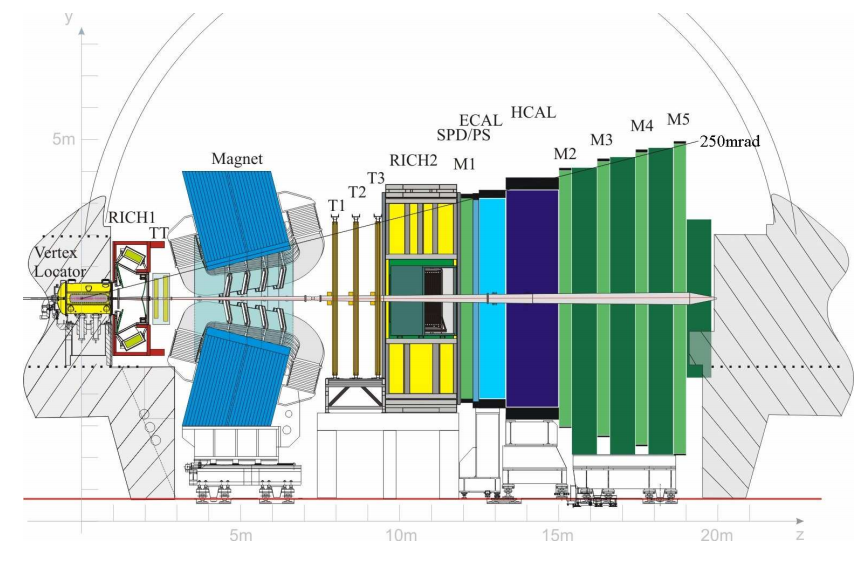
\includegraphics[width=0.8\textwidth]{graphics/lhcb.png}
  \caption{Components of the LHCb detector. \cite{lhcb}}
  \label{fig:lhcb}
\end{figure}

The Vertex Locator (VELO) consists of several silicon modules and is constructed to measure the location of the proton-proton collision vertex as well as secondary $B$ meson vertices.
This is neccessary because due to the relatively long lifetime and therefore relatively large flight distances of $B$ mesons.
TT, T1, T2 and T3 are the silicon tracking detectors build to reconstruct particle tracks.
T1-T3 also contain tube modules filled with a mixture of argon and carbondioxide.
These gases are being ionized by particles resulting in a measurable signal.
To get the particles' momenta, a magnet with an integrated magnetic field of $\SI{4}{\milli\tesla}$ is used to measure the curvature of the charged partilce's tracks.
This curvature determines the momentum of each charged particle.
To lower systematic uncertainties, the polarity of this magnet is reversed frequently.
The Cherenkov detectors RICH1 and RICH2 give information about the particle velocity using the cherenkov effect.
RICH1 gives information about low momentum charged particles using aeorgel and $\text{C}_4\text{F}_{10}$ radiators while RICH2 gives information about high momentum charged particles using a $\text{CF}_4$ radiator.
Combining the information of momentum and velocity can determine the mass of a particle.
The calorimetersystem consists of a scintillating pad (SPD), a preshower detector (PS), an electromagnetic calorimeter (ECAL) and a hadronic calorimeter (HCAL).
Here most of the particles (with the exception of muons) deposit all their energy.
The shower cluster of the deposited energy gives more information on which particle has been detected.
Since muons are minimal ionizing particles, they cannot be stopped in the calorimeters.
Therefore muon chambers are installed consisting of five stations (M1-M5).


To reduce the amount of data taken, a trigger system is used.
The trigger system consists of a hardware component and a software component.
The hardware component uses information from the calorimeters and muon chambers while the software component reconstructs the event in real time and decides if the event is from interest.
